\section{Материалы предварительного проектирования системы}
\subsection{Функциональная схема обработки данных}

\begin{figure}[!htb]
    \centering
    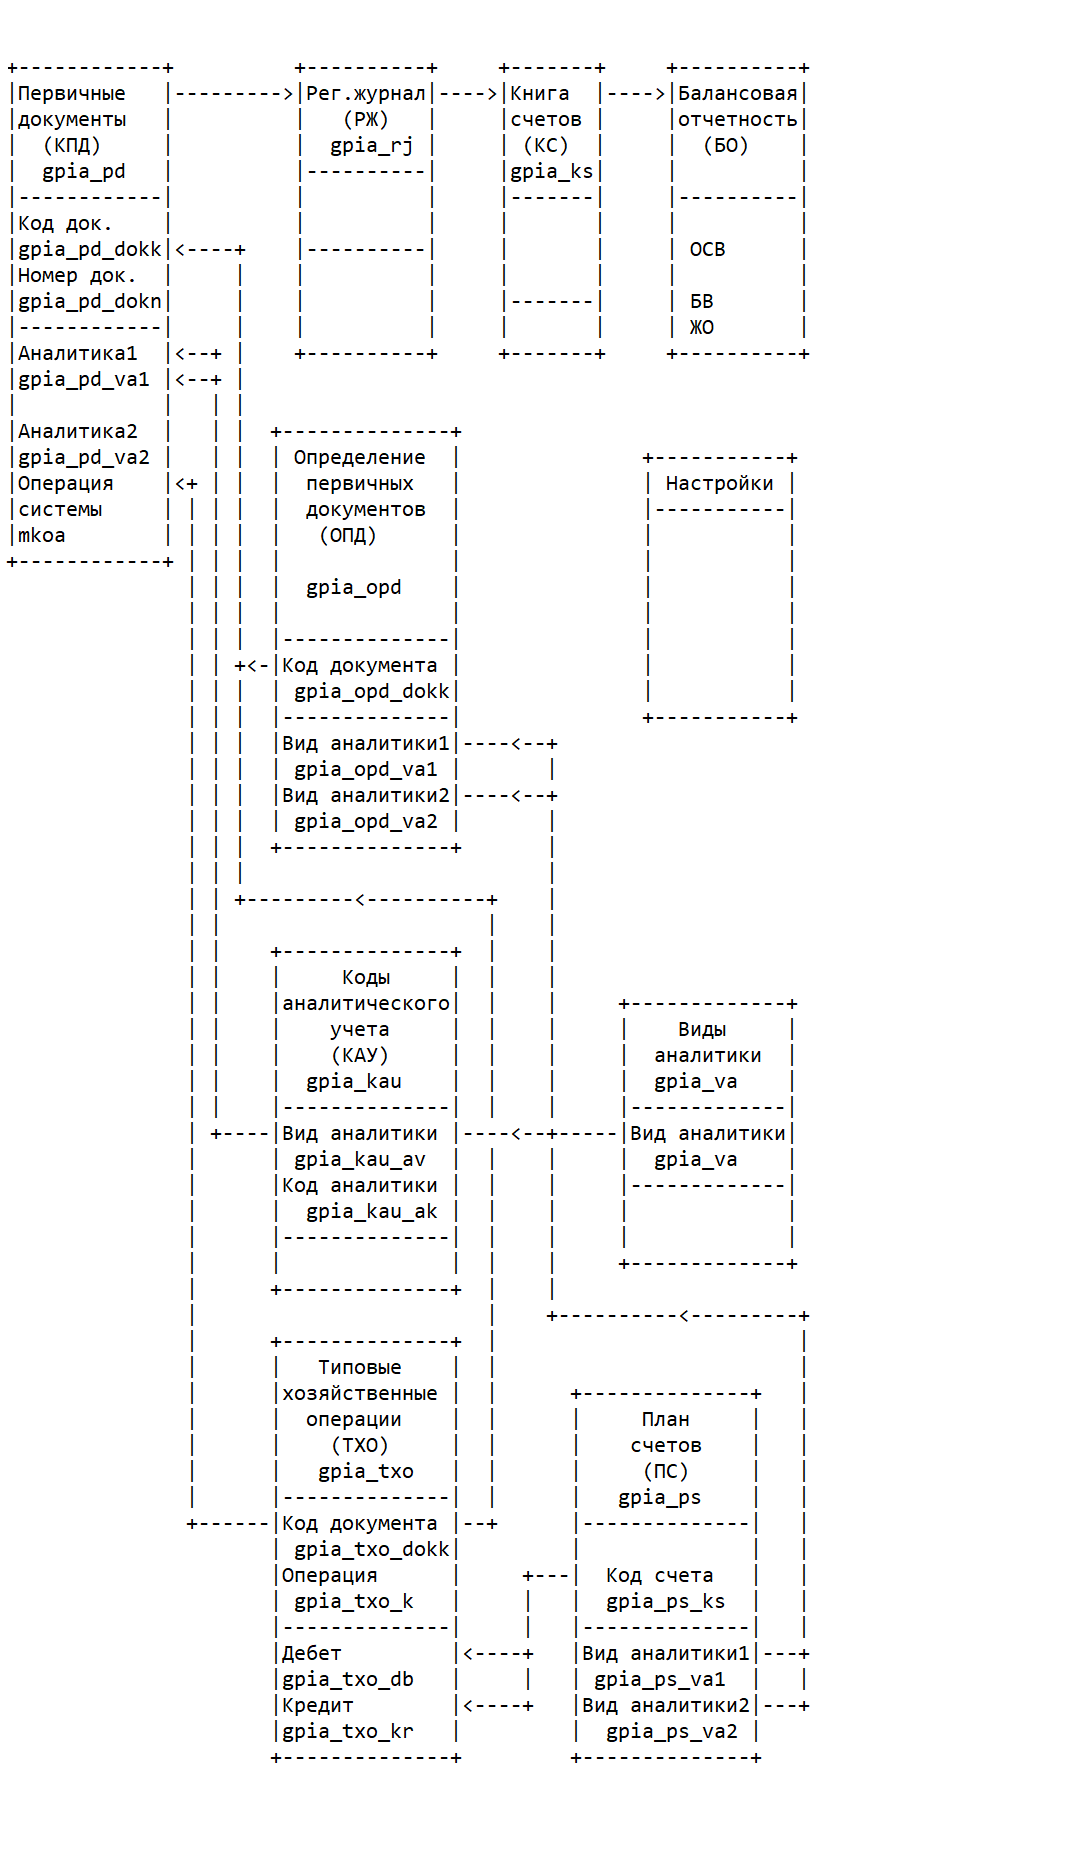
\includegraphics[height=19cm]
        {_assets/gpia_part2.png}
    \caption{Функциональная схема обработки данных}
    \label{fig:gpia_part2}
\end{figure}

\subsection{Описание картотек}

Картотеки:

\begin{itemize}
    \item Первичные документы gpia\_pd;
    \item[]\hspace{0pt}
    \item Регистрационный журнал (РЖ) gpia\_rj;
    \item Книга счетов (КС) gpia\_ks;
    \item[]\hspace{0pt}
    \item Определение первичных документов gpia\_opd;
    \item Типовые хозяйственные операции (ТХО) gpia\_txo;
    \item План счетов (ПС) gpia\_ps;
    \item Коды аналитического учёта (КАУ) gpia\_kau;
    \item Виды аналитики gpia\_va;
    \item[]\hspace{0pt}
    \item Настройки системы gpia\_nst;
\end{itemize}

\begin{table}[h!p]
    \centering
    \scriptsize
    \caption{Первичные документы gpia\_pd}
    \begin{tabular}{|l|l|l|} 

\hline
\textbf{Реквизит}                   &\textbf{Обозначение}&\textbf{Тип и значность}  \\ \hline
поле связи               =0         &gpia\_pd\_0        &c1                         \\ \hline
код документа    < --- opd          &gpia\_pd\_dokk     &c3                         \\ \hline
номер документа                     &gpia\_pd\_dokn     &n5                         \\ \hline
дата документа                      &gpia\_pd\_dokd     &D                          \\ \hline
вид аналитики 1    *opd             &gpia\_pd\_av1      &c3                         \\ \hline
тип аналитики 1      =д, к, x       &gpia\_pd\_avt1     &c1                         \\ \hline
аналитика код 1   < --- kau         &gpia\_pd\_ak1      &c10                        \\ \hline
вид аналитики2                      &gpia\_pd\_av2      &c3                         \\ \hline
тип аналитики2                      &gpia\_pd\_avt2     &c1                         \\ \hline
аналитика код2                      &gpia\_pd\_ak2      &c10                        \\ \hline
вид аналитики3                      &gpia\_pd\_av3      &c3                         \\ \hline
тип аналитики3                      &gpia\_pd\_avt3     &c1                         \\ \hline
аналитика код3                      &gpia\_pd\_ak3      &c10                        \\ \hline
операции                            &gpia\_pd\_to       &c10                        \\ \hline
дебет счет *txo                     &gpia\_pd\_db       &n2                         \\ \hline
дебет счет субсчет наименование *txo&gpia\_pd\_dbn      &c10                        \\ \hline
кредит  *txo                        &gpia\_pd\_kr       &n2                         \\ \hline
кредит название*txo                 &gpia\_pd\_krn      &c10                        \\ \hline
сумма                               &gpia\_pd\_rub      &n8                         \\ \hline
SAE                                 &gpia\_pd\_sae      &c10                        \\ \hline

    \end{tabular}
\end{table}

\begin{table}[h!p]
    \centering
    \scriptsize
    \caption{Виды аналитики gpia\_va}
    \begin{tabular}{|l|l|l|} 

                                                                               \hline
\textbf{Реквизит}       &\textbf{Обозначение}   &\textbf{Тип и значность}   \\ \hline
поле связи  	  =0    &gpia\_va\_0            &c1                         \\ \hline
вид аналитики           &gpia\_va\_k            &c3                         \\ \hline
название вида аналитики &gpia\_va\_n            &c15                        \\ \hline

    \end{tabular}
\end{table}

\begin{table}[h!p]
    \centering
    \scriptsize
    \caption{Регистрационный журнал (РЖ) gpia\_rj}
    \begin{tabular}{|l|l|l|} 

                                                                                   \hline
\textbf{Реквизит}           &\textbf{Обозначение}   &\textbf{Тип и значность}   \\ \hline
поле связи	=0              &gpia\_rj\_0            &c1                         \\ \hline
дата операции               &gpia\_rj\_data         &D                          \\ \hline
код оправдательного документа&gpia\_rj\_dokk        &c3                         \\ \hline
номер документа             &gpia\_rj\_dokn         &n5                         \\ \hline
дата документа              &gpia\_rj\_dokd         &D                          \\ \hline
содержание операции         &gpia\_rj\_to           &c10                        \\ \hline
дебет, счет                 &gpia\_rj\_db           &n2                         \\ \hline
дебет, название             &gpia\_rj\_dbn          &c10                        \\ \hline
кредит, счет                &gpia\_rj\_kr           &n2                         \\ \hline
кредит название             &gpia\_rj\_krn          &c10                        \\ \hline
SAE                         &gpia\_rj\_sae          &c10                        \\ \hline
Сумма                       &gpia\_rj\_rub          &n10                        \\ \hline

    \end{tabular}
\end{table}

\begin{table}[h!p]
    \centering
    \scriptsize
    \caption{Книга счетов(КС) gpia\_ks}
    \begin{tabular}{|l|l|l|} 

                                                                                   \hline
\textbf{Реквизит}           &\textbf{Обозначение}   &\textbf{Тип и значность}   \\ \hline
поле связи  =0              &gpia\_ks\_0      &c1                                 \\ \hline
дата операции               &gpia\_ks\_data   &D                                  \\ \hline
код оправдательного документа&gpia\_ks\_dokk  &c3                                 \\ \hline
номер документа             &gpia\_ks\_dokn   &n5                                 \\ \hline
дата документа              &gpia\_ks\_dokd   &D                                  \\ \hline
операции                    &gpia\_ks\_to     &c10                                \\ \hline
счет                        &gpia\_ks\_s      &n2                                 \\ \hline
счёт название               &gpia\_ks\_sn     &c10                                \\ \hline
кор. счёт                   &gpia\_ks\_ks     &n2                                 \\ \hline
кор. счет наименование      &gpia\_ks\_ksn    &c10                                \\ \hline
сумма дб                    &gpia\_ks\_db     &n10                                \\ \hline
сумма кр                    &gpia\_ks\_kr     &n10                                \\ \hline
SAE                         &gpia\_ks\_sae    &c10                                \\ \hline

    \end{tabular}
\end{table}

\begin{table}[h!p]
    \centering
    \scriptsize
    \caption{Определение первичных документов gpia\_opd}
    \begin{tabular}{|l|l|l|} 

                                                                                   \hline
\textbf{Реквизит}           &\textbf{Обозначение}   &\textbf{Тип и значность}   \\ \hline
поле связи       =0         &gpia\_opd\_0           &c1                         \\ \hline
код документа               &gpia\_opd\_k           &c3                         \\ \hline
наименование документа      &gpia\_opd\_n           &c10                        \\ \hline
вид аналитики 1  < ---  va  &gpia\_opd\_av1         &c3                         \\ \hline
тип аналитики 1    =д, к, x &gpia\_opd\_avt1        &c1                         \\ \hline
виды аналитики 2            &gpia\_opd\_av2         &c3                         \\ \hline
тип аналитики 2             &gpia\_opd\_avt2        &c1                         \\ \hline
вид аналитики 3             &gpia\_opd\_av3         &c3                         \\ \hline
тип аналитики 2             &gpia\_opd\_avt3        &c1                         \\ \hline

    \end{tabular}
\end{table}

\begin{table}[h!p]
    \centering
    \scriptsize
    \caption{Типовые хозяйственные операции(ТХО) gpia\_txo}
    \begin{tabular}{|l|l|l|} 

                                                                                           \hline
\textbf{Реквизит}                   &\textbf{Обозначение}   &\textbf{Тип и значность}   \\ \hline
поле связи    =0                    &gpia\_txo\_0           &c1                         \\ \hline
код документа        < ---  opd     &gpia\_txo\_dokk        &c3                         \\ \hline
Операции                            &gpia\_txo\_k           &c10                        \\ \hline
дебет, счёт            < ---  ps\_1 &gpia\_txo\_db          &n2                         \\ \hline
дебет, название       * ps\_1       &gpia\_txo\_dbn         &c10                        \\ \hline
кредит                   < --- ps\_2&gpia\_txo\_kr          &n2                         \\ \hline
кредит, название    * ps\_2         &gpia\_txo\_krn         &c10                        \\ \hline
SAE                                 &gpia\_txo\_sae         &c10                        \\ \hline

    \end{tabular}
\end{table}

\begin{table}[h!p]
    \centering
    \scriptsize
    \caption{План счетов(ПС) gpia\_ps}
    \begin{tabular}{|l|l|l|} 

                                                                                           \hline
\textbf{Реквизит}                   &\textbf{Обозначение}   &\textbf{Тип и значность}   \\ \hline
поле связи        =0                &gpia\_ps\_0            &c1                         \\ \hline
счет                                &gpia\_ps\_s            &n2                         \\ \hline
название счета                      &gpia\_ps\_n            &c10                        \\ \hline
тип счета          = а, п, x        &gpia\_ps\_typ          &c1                         \\ \hline
вид аналитики 1 из VA               &gpia\_ps\_av1          &c3                         \\ \hline
вид аналитики 2 из VA               &gpia\_ps\_av2          &c3                         \\ \hline

    \end{tabular}
\end{table}

\begin{table}[h!p]
    \centering
    \scriptsize
    \caption{Коды аналитического учёта(КАУ) gpia\_kau}
    \begin{tabular}{|l|l|l|} 

                                                                               \hline
\textbf{Реквизит}       &\textbf{Обозначение}   &\textbf{Тип и значность}   \\ \hline
поле связи          =0  &gpia\_kau\_0           &c1                         \\ \hline
вид аналитики           &gpia\_kau\_k           &c5                         \\ \hline
вид аналитики           &gpia\_kau\_n           &c15                        \\ \hline

    \end{tabular}
\end{table}

\begin{table}[h!p]
    \centering
    \scriptsize
    \caption{Настройки системы gpia\_nst}
    \begin{tabular}{|l|l|l|} 

                                                                               \hline
\textbf{Реквизит}       &\textbf{Обозначение}   &\textbf{Тип и значность}   \\ \hline
поле связи          =0  &gpia\_nst\_0           &c1                         \\ \hline
дата текущая            &gpia\_nst\_datat       &D                          \\ \hline
интервал с              &gpia\_nst\_datas       &D                          \\ \hline
интервал до             &gpia\_nst\_datado      &D                          \\ \hline
cчёт                    &gpia\_nst\_s           &n2                         \\ \hline
название счёта          &gpia\_nst\_sn          &c10                        \\ \hline
название фирмы          &gpia\_nst\_firma       &c10                        \\ \hline

    \end{tabular}
\end{table}

\subsection{Описание работ}

\begin{table}[h!p]
    \centering
    \scriptsize
    \caption{Описание работ}
    \begin{tabular}{|p{8cm}|p{9cm}|} 

% = = = = = = = = = =

\hline

% = = = = = = = = = =

\textbf{Группа работ}
&
\textbf{Работы}
\\ \hline

% = = = = = = = = = =

Формирование и разноска первичных документов \par
\hspace{0pt} \par
\textbf{gpia\_Документы}
&
- gpia\_Ввод текущей даты \par
- gpia\_Ввод и разноска первичных документов
\\ \hline

% = = = = = = = = = =

Работа с регистрационным журналом \par
\hspace{0pt} \par
\textbf{gpia\_РЖ}
&
- gpia\_Просмотр РЖ \par
- gpia\_Просмотр РЖ (запрос) \par
- gpia\_Формирование книги счетов из рег. журнала \par
- gpia\_Просмотр КС \par
- gpia\_Просмотр КС (запрос) \par
- gpia\_Печать книги счетов
\\ \hline

% = = = = = = = = = =

Формирование балансовой отчетности \par
\hspace{0pt} \par
\textbf{gpia\_БО}
&
- gpia\_Опеделение форм \par
- gpia\_Оборотно-сальдовая ведомость за период... по счету... \par
- gpia\_Балансовая ведомость по счету за период... по счету... \par
- gpia\_Журнал-ордер за период... по счету...
\\ \hline

% = = = = = = = = = =

Сопровождение картотек-справочников \par
\hspace{0pt} \par
\textbf{gpia\_Картотеки}
&
- gpia\_Определение первичных документов \par
- gpia\_Типовые хозяйственные операции(ТХО) \par
- gpia\_План счетов(ПС) \par
- gpia\_Виды аналитики \par
- gpia\_Коды аналитического учёта(КАУ) \par
- gpia\_Настройка АРМа
\\ \hline

% = = = = = = = = = =

Ведение архивов \par
\hspace{0pt} \par
\textbf{gpia\_Архивы}
&
- gpia\_Копирование системы!!! \par
- gpia\_Восстановление системы!!!
\\ \hline

% = = = = = = = = = =

Выход из системы \par
\hspace{0pt} \par
\textbf{gpia\_Выход}
&
- gpia\_Выход из системы
\\ \hline

% = = = = = = = = = =

    \end{tabular}
\end{table}

\newpage
